\section{Abstract}
Il progetto si propone di realizzare il sito web di un rivenditore di componenti per PC.
Lo scopo principale è quello di fornire ai clienti una interfaccia dalla quale possono visualizzare e ordinare i pezzi che vogliono acquistare, il sito quindi offre la classica funzionalità di \emph{carrello}, dove l'utente può inserire i componenti che vorrebbe acquistare, inoltre per ogni utente è disponibile la storia degli acquisti effettuati, da questa lista l'utente è in grado di dare una valutazione e di scrivere una recensione sul prodotto.
Un admin può aggiungere e rimuovere oggetti dal catalogo, e creare dei Bundle che verranno visualizzati nella Home.

\section{Utenti destinatari}
I clienti del negozio sono generalmente persone già informate su cosa vogliono acquistare e sulla funzione dei vari componenti, perciò vengono fornite le caratteristiche tecniche di ogni pezzo, gli utenti possono inoltre fare ricerche mirate sul nome di un componente oppure tramite una ricerca avanzata possono selezionare un tipo specifico di componenti (RAM,Processore,ecc...).
Per non lasciare fuori gli utenti meno esperti forniamo nella home page una serie di computer preassemblati su diverse fasce di prezzo con una semplice descrizione che aiuti i clienti meno esperti a capire se una data macchina soddisfa o meno i suoi bisogni.
\newpage
\section{Mappa del Sito}
\subsection{Utente non registrato}
\begin{figure}[h]
	\label{UNR} 
	\centering 
	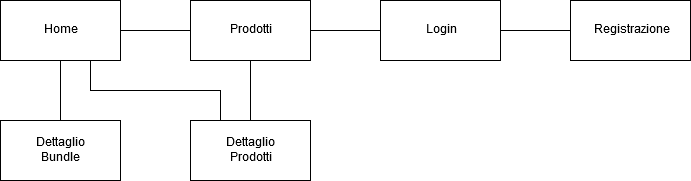
\includegraphics[width=1\textwidth]{immagini/UNR.png}
	\caption{Mappa del sito per un utente non registrato} 
\end{figure}
Un utente non registrato è in grado di visualizzare la home e i prodotti presenti nel sito, può inoltre registrarsi come utente comune oppure se ha già delle credenziali più effettuare il login.

\subsection{Utente registrato}
\begin{figure}[h]
	\label{UR} 
	\centering 
	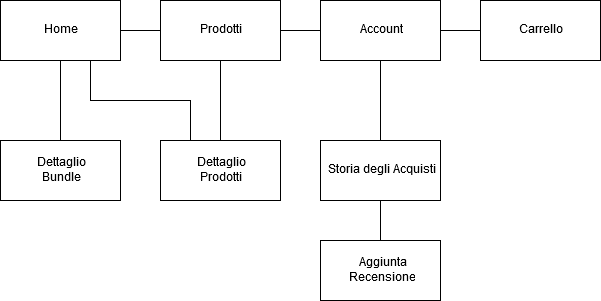
\includegraphics[width=1\textwidth]{immagini/UR.png}
	\caption{Mappa del sito per un utente registrato} 
\end{figure}
Un utente registrato oltre a visualizzare i prodotti presenti nel sito è in grado di aggiungerli al carrello personale ed effettuare l'acquisto.
Questo tipo di utente può visualizzare i prodotti acquistati in passato e aggiungere una recensione ad essi, può inoltre effettuare il logout in ogni momento.

\subsection{Admin}
\begin{figure}[h]
	\label{figuragattino} 
	\centering % centra
	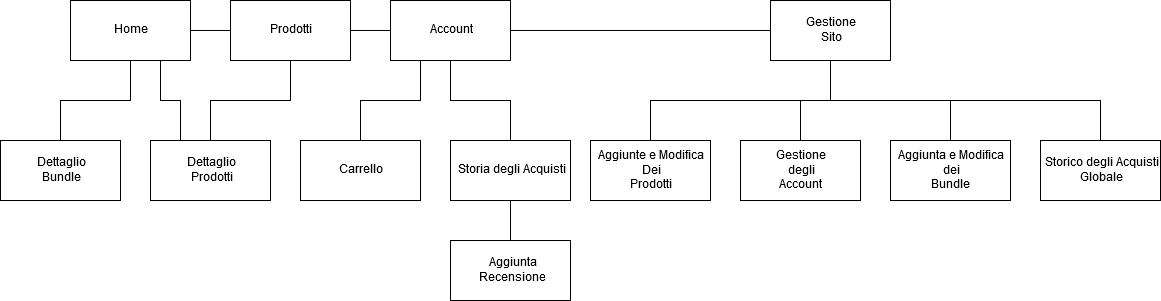
\includegraphics[width=1\textwidth]{immagini/admin.png}
	\caption{Mappa del sito per un admin} 
\end{figure}
Un admin è in grado di fare tutto ciò che può fare un normale utente ma è anche in grado di accedere alla pagina di gestione del sito dalla quale è possibile aggiungere nuovi prodotti, gestire gli account dei vari utenti, modificare i bundle e visualizzare lo storico degli acquisti effettuati sul sito da tutti gli utenti.